\documentclass[a4paper, 12pt]{report}
\usepackage[french]{babel}
\usepackage[utf8]{inputenc}
\usepackage[T1]{fontenc}
\usepackage{graphicx}
\usepackage{geometry}
\usepackage{tabularx}
\usepackage{caption}
\usepackage{amsmath}
%\usepackage[usenames,dvipsnames,svgnames,table]{xcolor}
%\usepackage{pdfpages}
%\geometry{hmargin=2.5cm,vmargin=2.5cm}

% Title Page
\begin{document}
\begin{titlepage}
\newcommand{\HRule}{\rule{\linewidth}{0.5mm}}

\begin{center}

\HRule \\[0.4cm]
{ \huge Projet : Exécution symbolique et tests structurels}\\[0.4cm]
\HRule \\[2cm]

\vspace{2cm}

Ayaz Badouraly \& Venceslas Danguy des Déserts

\vspace{2cm}

Enseignante :
Mme Pascale Le Gall


\end{center}
\end{titlepage}

%\maketitle
%\newpage


\tableofcontents
\newpage

\chapter{Architecture du projet}

\section{Pipe de traitement}

Le code se divise en trois grandes parties : parsing du programme dans le langage WHILE, vérification de critères sur ce programme, génération des tests pour les critères.

\subsection{Parsing}

Le parsing consiste, à partir d'un programme écrit en langage WHILE, à obtenir un graphe de contrôle (CFG) représentant le dit programme. On passe pour cela par une étape intermédiaire : un arbre de syntaxe abstraite, ou AST. L'AST est une représentation du code du programme sous forme d'arbre, tandis que le CFG représente vraiment le flux du programme.

%Insérer exemples AST et CFG associés

\subsubsection{Génération de l'AST}

Nous utilisons pour ce faire la librairie Python ply, qui fournit une implémentation en Python du duo lex/yacc. Lex tokenize le programme en entrée en fonction de la grammaire définie, tandis que yacc prend l'entrée tokenizée et fournit l'AST. Nous utilisons la librairie \textit{anytree} pour manipuler les arbres.

\subsubsection{Conversion de l'AST au CFG}

Il faut ensuite traduire cet AST en CFG. On utilise pour cela un algorithme récursif qui va parcourir l'arbre et construire le CFG. Chaque exécution de la fonction récursive renvoie un morceau de graphe ainsi que des arêtes sortantes à relier.

Ainsi, la conversion d'un arbre ne contenant en tout et pour tout qu'une assignation va renvoyer un noeud labellisé et une arête sortante de ce noeud portant une condition \textit{True} et une commande \textit{Assign}.

La conversion d'un arbre contenant un noeud While va relier les arêtes sortantes du graphe du sous-arbre au noeud parent de façon à former une boucle, etc.

On ajoute enfin un tag sur les noeuds correspondant à des instructions \textit{If} ou \textit{While} pour faciliter la vérification et la génération des tests.

Les graphes sont gérés par la librairie python \textit{networkx}.

\subsection{Vérification de critères}

Nous sommes donc désormais capables d'obtenir le CFG associé à un programme écrit en langage WHILE. Nous voulons maintenant \textit{vérifier} des critères de tests pour ce programme, c'est à dire, étant donné un jeu de tests (données de départs), dire si les tests couvrent un ensemble de cas (chemins d'exécution) précis.

Il faut donc commencer par exécuter le programme avec le jeu de test. Ceci se fait assez facilement, il suffit de parcourir le graphe de contrôle en maintenant un état (ensemble des variables et de leurs valeurs) et en choisissant, à chaque branchement, l'arête dont la condition est vérifiée par l'état.

On obtient ainsi un ensemble de chemins d'exécution (un par valuation de départ).

Parallèlement, on a un critère de test, c'est à dire un ensemble de chemins par lesquels nous voulons passer. Ainsi le critère \textit{Toutes les affectations} demande-t-il qu'à la fin de l'exécution de tous les tests, on soit passé au moins une fois par chaque arête portant une commande \textit{Assign}.

Chaque critère possède son propre algorithme de génération d'éléments à vérifier en fonction du programme (bien que l'on puisse toujours se ramener à un ensemble de chemins, il était parfois plus simple de considérer un ensemble de noeuds ou d'arêtes par lesquels il faut passer).

Il suffit ensuite de faire l'intersection des deux ensembles \textit{\{Chemins exécutés lors de la phase du test\}} et \textit{\{Chemins à vérifier imposés par le critère\}}.


\section{Choix de conception}

\section{Limitations adoptées}

\section{Organisation du code}

Le code est organisé en modules.

\begin{description}
\item[- astree :] Contient notre structure d'AST avec les commandes et opérations définies par la sémantique opérationnelle de WHILE.
\item[- cfgraph :] Code utilisé pour exécuter un test sur le programme. Le module utils, en particulier, contient toutes les fonctions du graphe nécessaires pour générer les éléments à vérifier pour chaque critère.
\item[- syntax :] Contient le code du lexeur et du parseur ainsi que leur configuration
\item[- tests :] Ce dossier contient le coeur du projet. Le module \textit{tester} contient la logique de vérification des critères : récupération des éléments à vérifier, analyse des chemins d'exécutions des tests pour y trouver les éléments. Le module \textit{generator} gère la génération des jeux de tests en faisant appel au solveur \textit{Z3}.
\item[- utils :] Contient notamment la conversion de l'AST vers le CFG.
\item[- input :] Contient des exemples de programmes sur lesquels on peut vérifier les critères.
\item[- output :] Exemples de graphes (images).
\end{description}

\chapter{Vérification des critères}
% D'après le sujet, pour chaque critère :
% - Jeux de tests satisfaisant et ne satisfaisant pas le critère
% - Mécanisme de vérification
% - Mécanisme de génération
% Et en général : relations d'ordre entre les critères

\section{Toutes les affectations}
\label{sec:affectations}
On va travailler sur le programme suivant :

\begin{minipage}{0.46\textwidth}
\begin{verbatim}
1:  if (X <= 0) {
2:      X := -X;
    } else {
3:      X := 1 - X;
    }

4:  if (X == 1) {
5:      X := 1;
    } else {
6:      X := X + 1;
    }
\end{verbatim}
\end{minipage}
\begin{minipage}{0.46\textwidth}
	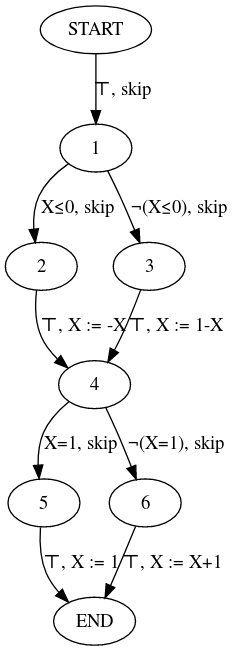
\includegraphics[scale=0.5]{pics/simpleCFG.png}
	\captionof{figure}{CFG associé}
\end{minipage}

%Ajouter AST + CFG en illustration de la partie précédente

Le critère \textit{Toutes les affectations} demande à ce que tous les labels d'affectations (ici : $2, 3, 5, 6$) apparaissent au moins une fois dans l'un des chemins d'exécution correspondant aux données de tests.

Si on prend pour jeu de test :

\[ \{
	\{ X : -1\},
	\{ X : 1\}
\} \]

On obtient les chemins d'exécutions suivants :
\begin{description}
\item[$\{ X : -1\}$ : ] $1, 2, 4, 5$
\item[$\{ X : 1\}$ : ] $1, 3, 4, 6$
\end{description}

On est donc passé au moins une fois par chaque label associé à une affectation : le critère est vérifié sur ce programme et ce jeu de test.

Si, en revanche, on s'était contenté d'un unique test $\{ X : -1\}$, on ne serait pas passé par les noeuds $3$ et $6$, et le critère n'aurait pas été vérifié.

Dans la pratique, étant donné un CFG, on récupère l'ensemble des noeuds (labels) tels qu'une arête sortante de ce noeud porte une affectation. Ceci se fait très facilement en parcourant l'ensemble des arêtes (sans notion de chemin ici).
Il suffit ensuite de regarder lesquels de ces noeuds sont (ou non) dans les chemins des tests.

\section{Toutes les décisions}

On travaille toujours sur le programme défini en \ref{sec:affectations}.

Le critère \textit{Toutes les décisions} demande à ce que l'on passe au moins une fois par toutes les arêtes associées à une expression booléenne. Il s'agit, en bref, de toutes les arêtes sortantes des noeuds \textit{if} et \textit{while}, ce qui est équivalent à dire qu'il faut passer par les noeuds de destination de ces arêtes.

Ici, il faut donc passer par les noeuds $2, 3, 5, 6$. On retombe dans ce cas très simple sur les même éléments que le critère \textit{Toutes les affectations}, et le même jeu de tests vérifie donc les deux critères.

\section{Tous les \textit{k}-chemins}

Ce critère demande que chaque chemin d'exécution de longueur inférieure ou égale à $k$ soit exécuté.

On commence donc par implémenter un générateur qui va renvoyer tous les chemins correspondants. Pour ce faire, on réalise un parcours en profondeur du graphe, où l'on s'arête lorsqu'on à un chemin complet (noeud \textit{END} atteint) ou lorsque l'on a atteint la longueur maximale $k$.

Une fois que l'on a l'ensemble des chemins à vérifier, il suffit de comparer cet ensemble avec celui des chemins exécutés par les tests.

Sur le programme de la partie \ref{sec:affectations}, pour le critère \textit{Tous les 10-chemins}, il faut vérifier les chemins suivants (en fait, tous, car on a pris $k$ grand):

\begin{align*}
\{
	&[START, 1, 2, 4, 5, END],\\
	&[START, 1, 2, 4, 6, END],\\
	&[START, 1, 3, 4, 5, END],\\
	&[START, 1, 3, 4, 6, END]
\}
\end{align*}

On note que le chemin $[START, 1, 3, 4, 5, END]$ n'est pas faisable. Malheureusement, cela ne peut se détecter qu'à l'étape de génération des tests  : d'où l'importance de signaler à l'utilisateur quels sont les chemins manquants afin qu'il puisse décider de lui-même si ou non la couverture peut-être améliorée en complétant le jeu de tests.

Le jeu de tests suivant permet d'atteindre la couverture maximale :

\[ \{
	\{ X : -1\},
	\{ X : 1\};
	\{ X : 3\},
\} \]


\section{Toutes les \textit{i}-boucles}
\section{Toutes les définitions}

Le critère \textit{Toutes les définitions} demande que, pour chaque variable $X$, pour chaque noeud $u$ affectant $X$, on ait un chemin $..u...v..$ tel que $v$ utilise $X$, et qu'il n'y ait pas de réaffectation de $X$ entre $u$ et $v$.

Pour vérifier ce critère, nous commençons par implémenter les fonctions \textit{def} et \textit{ref} telles que définies dans l'énoncé.

On construit ensuite un dictionnaire \textit{definitions} qui associe à chaque variable $X$ l'ensemble des noeuds u tels que $X \in def(u)$.

Pour chaque variable $X$, on regarde ensuite chaque chemin. Si on trouve un noeud $u$ intéressant, c'est à dire $X \in def(u)$, on suit le chemin jusqu'à trouver $v$ tel que $X \in ref(v)$. On s'assure bien sûr qu'entre $u$ et $v$, il n'y a pas de noeud $u'$ tel que $X \in ref(u')$. Si on trouve $v$, on supprime $u$ de $\textit{definitions}[X]$.

Si à la fin, \textit{definitons} est vide, alors le critère est vérifié.

Le programme de la partie \ref{sec:affectations} ne pourra jamais vérifier ce critère, quel que soit le jeu de test, car les affectations $5$ et $6$ ne sont jamais utilisées. Si on rajoute une commande print qui affiche une variable, ainsi qu'une nouvelle variable $Y$, on peut le réécrire :


\begin{verbatim}
1:  if (X <= 0) {
2:      X := -X;
3:		Y := 5;
    } else {
4:      X := 1 - X;
    }

5:  if (X == 1) {
6:      X := 1;
    } else {
7:      X := X + 1;
8:		print(Y);
    }
9: print(X);
\end{verbatim}

Le dictionnaire \textit{definitions} s'écrit alors :

\[ \{
	X : [2, 4, 6, 7],
	Y : [3]
\} \]

Le jeu de tests suivant ne vérifie pas le critère :

\[ \{
	\{ X=1, Y=1\},
	\{ X=-1, Y=1 \}
\} \]

(Pas de chemin entre 3 et 8)


Contrairement à cet autre jeu de tests :

\[ \{
	\{ X=1, Y=1\},
	\{ X=-2, Y=1 \}
\} \]

\section{Toutes les utilisations}

Le critère \textit{Toutes les utilisations} demande que toutes ls utilisations acessibles pour chaque définitions soient exécutées au moins une fois.

On crée en parcourant le graphe un dictionnaire \textit{usages} qui pour chaque variable $X$, associe à chaque noeud $u$ définissant $X$ ($X \in def(u)$) l'ensemble des noeuds $v$ successeurs de $u$ tels que $v$ utilise $X$ ($X \in ref(v)$) tels qu'il n'y ait pas de noeud $u'$ qui redéfinisse X sur le chemin de $u$ à $v$.

On modifie le programme pour mieux montrer ce critère :
\begin{verbatim}
1:  if (X <= 0) {
2:      X := -X;
    } else {
3:      X := 1 - X;
    }

4:  if (X == 1) {
5:      X := 1;
    } else {
6:      X := X + 1;
7: 		print(X);
    }
\end{verbatim}

Le dictionnaire \textit{usages} s'écrit :

\begin{align*}
usages = \{
			X : \{ &\\
		&2 : 4, \\
		&3 : 4, \\
		&6 : 7,	\}\}
\end{align*}

Un jeu de test vérifiant ce critère pour ce programme est alors :

\begin{align*}
\{
	\{ X : 0 \},
	\{ X : 1 \}
\}
\end{align*}

Notons que contrairement au critère \textit{Toutes les définitions}, le critère \textit{Toutes les utilisations} n'impose pas l'existence d'une utilisation !

\section{Tous les DU-chemins}

Tous les chemins simples entre une définition de $X$ et une utilisation de $X$ sans redéfinition doivent être exécutés au moins une fois.

Le critère \textit{Toutes les utilisations} demandait simplement qu'au moins un chemin entre une paire (utilisation, définition) soit exécuté, ce critère-ci demande que tous les chemins simples le soient.

On récupère tous les chemins simples entre chaque noeud de définition ($def(u) \neq \emptyset$) et $END$ grâce à la librairie \textit{networkx}.

On regarde ensuite ces chemins à la recherche de paire $(u, v)$ telles que $u$ définit $X$, $v$ utilise $X$, et il n'y a pas de redéfinition de $X$ entre $u$ et $v$.

Lorsqu'on trouve une telle paire, on stocke le chemin entre $u$ et $v$ dans un dictionnaire \textit{du\_paths}.

Il suffit ensuite de chercher ces morceaux de chemins dans les chemins d'exécutions correspondants aux tests.
\section{Toutes les conditions}

\chapter{Génération des tests}

\section{Implémentation}

On adopte la stratégie générale suivante pour générer les tests associés à un
critère donné :

\begin{itemize}
	\item générer un ensemble de chemins par lesquels on veut passer --- en
	fonction du critère, on voudra passer par \textbf{tous} les chemins, ou
	par \textbf{au moins} un chemin
	\item pour chaque chemin, faire une exécution symbolique --- on notera
	l'utilisation de symboles \textbf{uniques} associés à chaque variable
	explicite ou implicite (~\textit{ie.} les registres \texttt{\_reg}, qui
	enregistrent les calculent intermédiaires~)
	\item chaque exécution symbolique fournit des contraintes entre les
	symboles : donner ces contraintes au solveur Z3
	\item obtenir un test associé à un chemin si le problème est satisfiable
\end{itemize}

\bigskip

L'exécution symbolique à partir d'un chemin sur le CFG ainsi que la résolution
du problème de contraintes sont effectuées dans le fichier
\texttt{src/tests/solver.py}.

\bigskip

La génération des chemins est propre à chaque critère et est détaillée
ci-dessous. Sauf explicitement dit, lorsque l'on dira que l'on génére tous les
chemins entre deux nodes, on sous-entendra \textit{tous les chemins simples}.
Il s'agit d'un choix tout à fait discutable, mais étant donné l'indécitabilité
du problème de la génération des tests, il faut de toute manière se fixer une
limite raisonnable.

\subsection{Toutes les affectations}

Le critère \textit{toutes les affectations} est un critère sur les nodes du
CFG. Pour chaque node \texttt{SAssign}, on va générer tous les chemins jusqu'à
ce node, en partant du node \texttt{START}.

On obtient un test pour un node lorsqu'on trouve au moins un chemin généré
faisable.

\subsection{Toutes les décisions}

Le critère \textit{toutes les décisions} est un critère sur les edges du CFG.
On souhaite passer par chaque edge sortant d'un node de type \texttt{SIF} ou
\texttt{SWHILE}. On peut donc se ramener à un critère d'accessibilité au node
de décision (~\texttt{CIF} ou \texttt{CWHILE}~). On génère tous les chemins
jusqu'au node, puis pour chaque chemin, on génère deux chemins : un chemin où
l'on a rajouté l'edge associé à la décision \texttt{true}, un autre chemin où
l'on a rajouté l'edge associé à la décision \texttt{false}.

On obtient un test pour un edge lorsqu'on trouve au moins un chemin généré
faisable.

\subsection{Tous les $k$-chemins}

\subsection{Toutes les $i$-boucles}

\subsection{Toutes les définitions}

\subsection{Toutes les utilisations}

\subsection{Tous les DU-chemins}

\section{Résultats}




\end{document}